\section{Evaluation of Preprocessing Pipelines and Heuristics}
\label{sec:which_preprocessing}
<<<<<<< HEAD
Results from these experiments are shown in Figure~\ref{fig:boxplot_corr_docs} (top: CLEF 2015; bottom: CLEF 2016). For each category of methods and combination of preprocessing and heuristics, we report their variability in terms of Spearman rank correlation with the human assessments\footnote{Results for Pearson and Kendall correlations are reported in the online appendix, but showed similar trends.}. We further report summary results across all understandability assessment methods and sentence ending heuristics for each of the preprocessing pipelines. Finally, we also report the inter-assessor correlation (last box) when multiple assessors provided judgements about the understandability of Web pages (details about this data in Section~\ref{sec:data}). This provides an indication of the range of variability and subjectiveness when assessing understandability, along with the highest correlation we measured between human assessors. 
=======
>>>>>>> origin/master

Results from experiments with different preprocessing pipelines and heuristics are shown in Figure~\ref{fig:boxplot_corr_docs} (top: CLEF 2015; bottom: CLEF 2016). For each category of methods and combination of preprocessing and heuristics, we report their variability in Spearman rank correlation with the human assessments\footnote{Results for Pearson and Kendall correlation measures are reported in the online appendix, but showed similar trends.}. We further report summary results across all understandability assessment methods and sentence ending heuristics for each of the preprocessing pipelines. Finally, we also report the inter-assessor correlation (last box) when multiple assessors provided judgements about the understandability of Web pages (see Section~\ref{sec:data} for details about this data). This provides an indication of the range of variability and subjectiveness when assessing understandability, along with the highest correlation we measured between human assessors. 
 
We first examined the correlations between human assessments and readability formulas. We found that the \textit{Naive} preprocessing resulted in the lowest correlations, regardless of readability formula and heuristics (although \textit{DoNotForcePeriod} performed better than \textit{ForcePeriod}). Using Justext or Boilerplate resulted in higher correlations with human understandability assessments, and the \textit{ForcePeriod} heuristic was shown to be better than \textit{DoNotForcePeriod}. These results confirm the speculations of Palotti et al.~\cite{palotti15}: they found these settings to produce lower variances in understandability estimations and thus hypothesised that they were better suited to the task.

Overall, among readability formulas, the best results (highest correlations) were obtained by SMOG and Dale-Chall Index (see Table~\ref{tab:top_corr_metrics}). Although no single setting outperformed the others in both collections, we found that the use of CLI and FRE with \textit{Justext} provided the most stable results across the collections, with correlation coefficients as high as the best ones in both collections.
These results confirmed the advice put forward by Palotti et al.~\cite{palotti15}, i.e. if using readability measures, then CLI should be preferred, along with an appropriate HTML extraction pipeline, regardless of the heuristic for sentence ending\footnote{We provide detailed plots to compare our results with Palotti's in the online appendix.}.

When considering methods beyond those based on readability formulas, we found that the highest correlations were archived by the regressors (MLR) and classifiers (MLC), independent of the preprocessing method used. For methods in these categories, correlations were only marginally influenced by preprocessing and heuristics, with the exception of regressors on CLEF 2015 that did exhibit not negligible variances. \todo{I think the text is not clear here: need to discuss.} 

A common trend when comparing preprocessing pipelines is that the Naive pipeline provided the weakest correlations with human assessments for CLEF 2016, regardless of estimation methods and heuristics. This result however was not confirmed for CLEF 2015, where the Naive preprocessing negatively influenced correlations for the readability formula category (RF), but not for other categories, although it was generally associated with larger variances on the correlation coefficients.


%For that, we present in Figure~\ref{fig:boxplot_corr_docs} the box plot of Spearman rank correlation metric divided by preprocessing alternative for CLEF eHealth 2015 and 2016\footnote{Due to space limitation, additional plots with Pearson and Kendall correlations are available online at \url{XYZ}.}.
%Figures~\ref{fig:boxplot_corr_docs_2015} and~\ref{fig:boxplot_corr_docs_2016} the box plot of different correlation metrics divided by preprocessing alternative for CLEF eHealth 2015 and 2016. 
%For instance, the very first box plot in the upper part of these figures shows the absolute Pearson's rank correlation of different readability metrics when using a combination of Naive and ForcePeriod as preprocessing steps.
%Boxes extend from the lower to upper quartile values of the data, with a line at the median. Whiskers extend from the box to show the range of the data. Flier points are those past the end of the whiskers, usually interpreted as outlier values.


%We also include in Figures~\ref{fig:boxplot_corr_docs_2015} and~\ref{fig:boxplot_corr_docs_2016} 
%We also include in Figure~\ref{fig:boxplot_corr_docs} boxes for the summary of the 3 preprocessing procedures to remove HTML, the use of HTML features, which is done without any preprocessing and the comparison with other human assessors. For CLEF eHealth 2015, we used as human assessments the additional assessments made by unpaid medical students and health consumers (see~\cite{palotti16b}), while for CLEF eHealth 2016 data, we randomly selected 100 pages that were assessed by another assessor. \mytodo{add at least another person doing assessments}.
%The correlations with human assessments provide important insights on how hard and subjective understandability assessments are.

\begin{figure*}[h!]
   \centering
   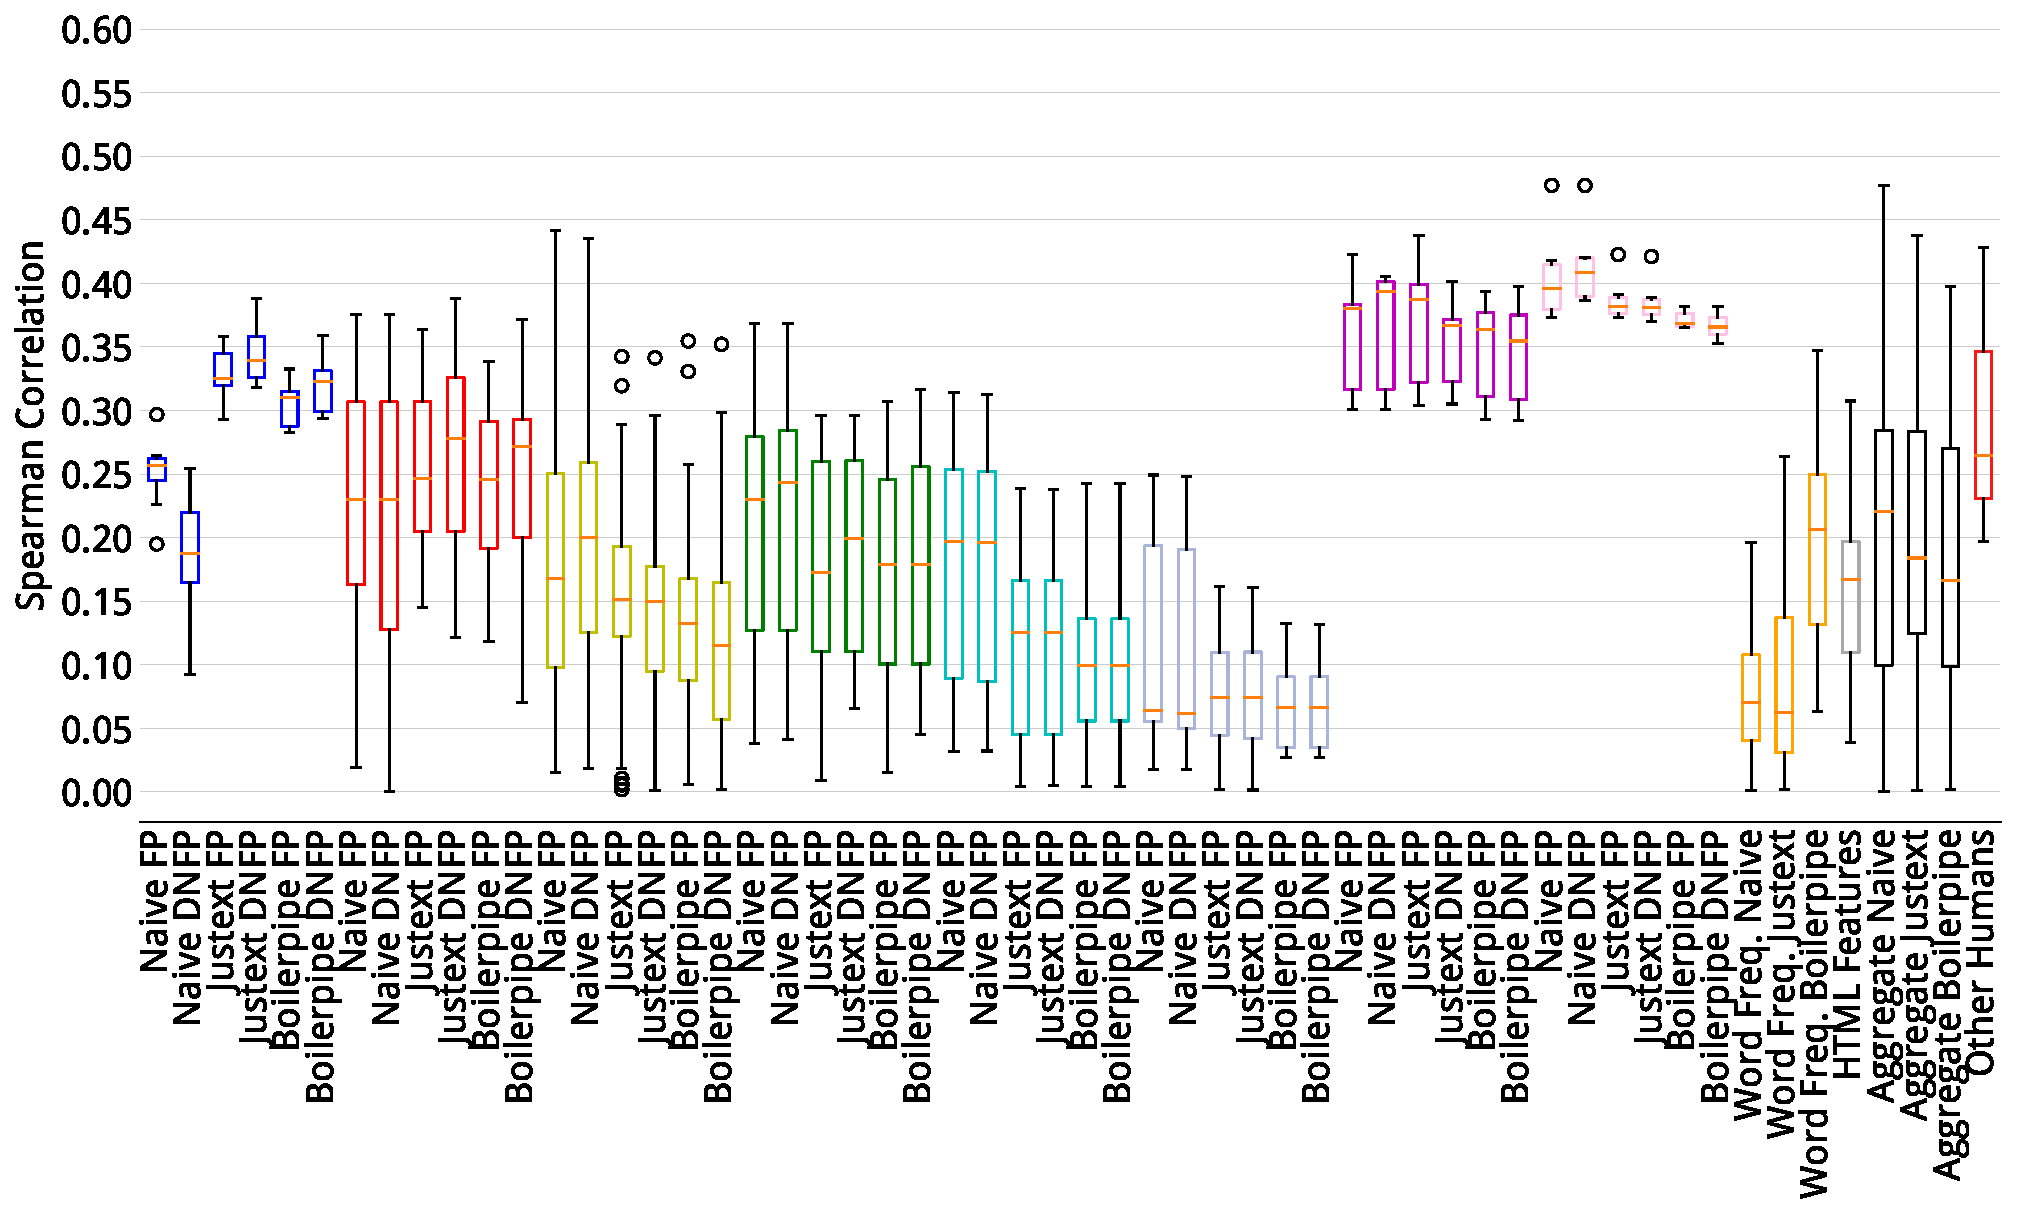
\includegraphics[width=0.6\textwidth]{graphics/box_spearman15_raw_values}\vspace{-7pt}
   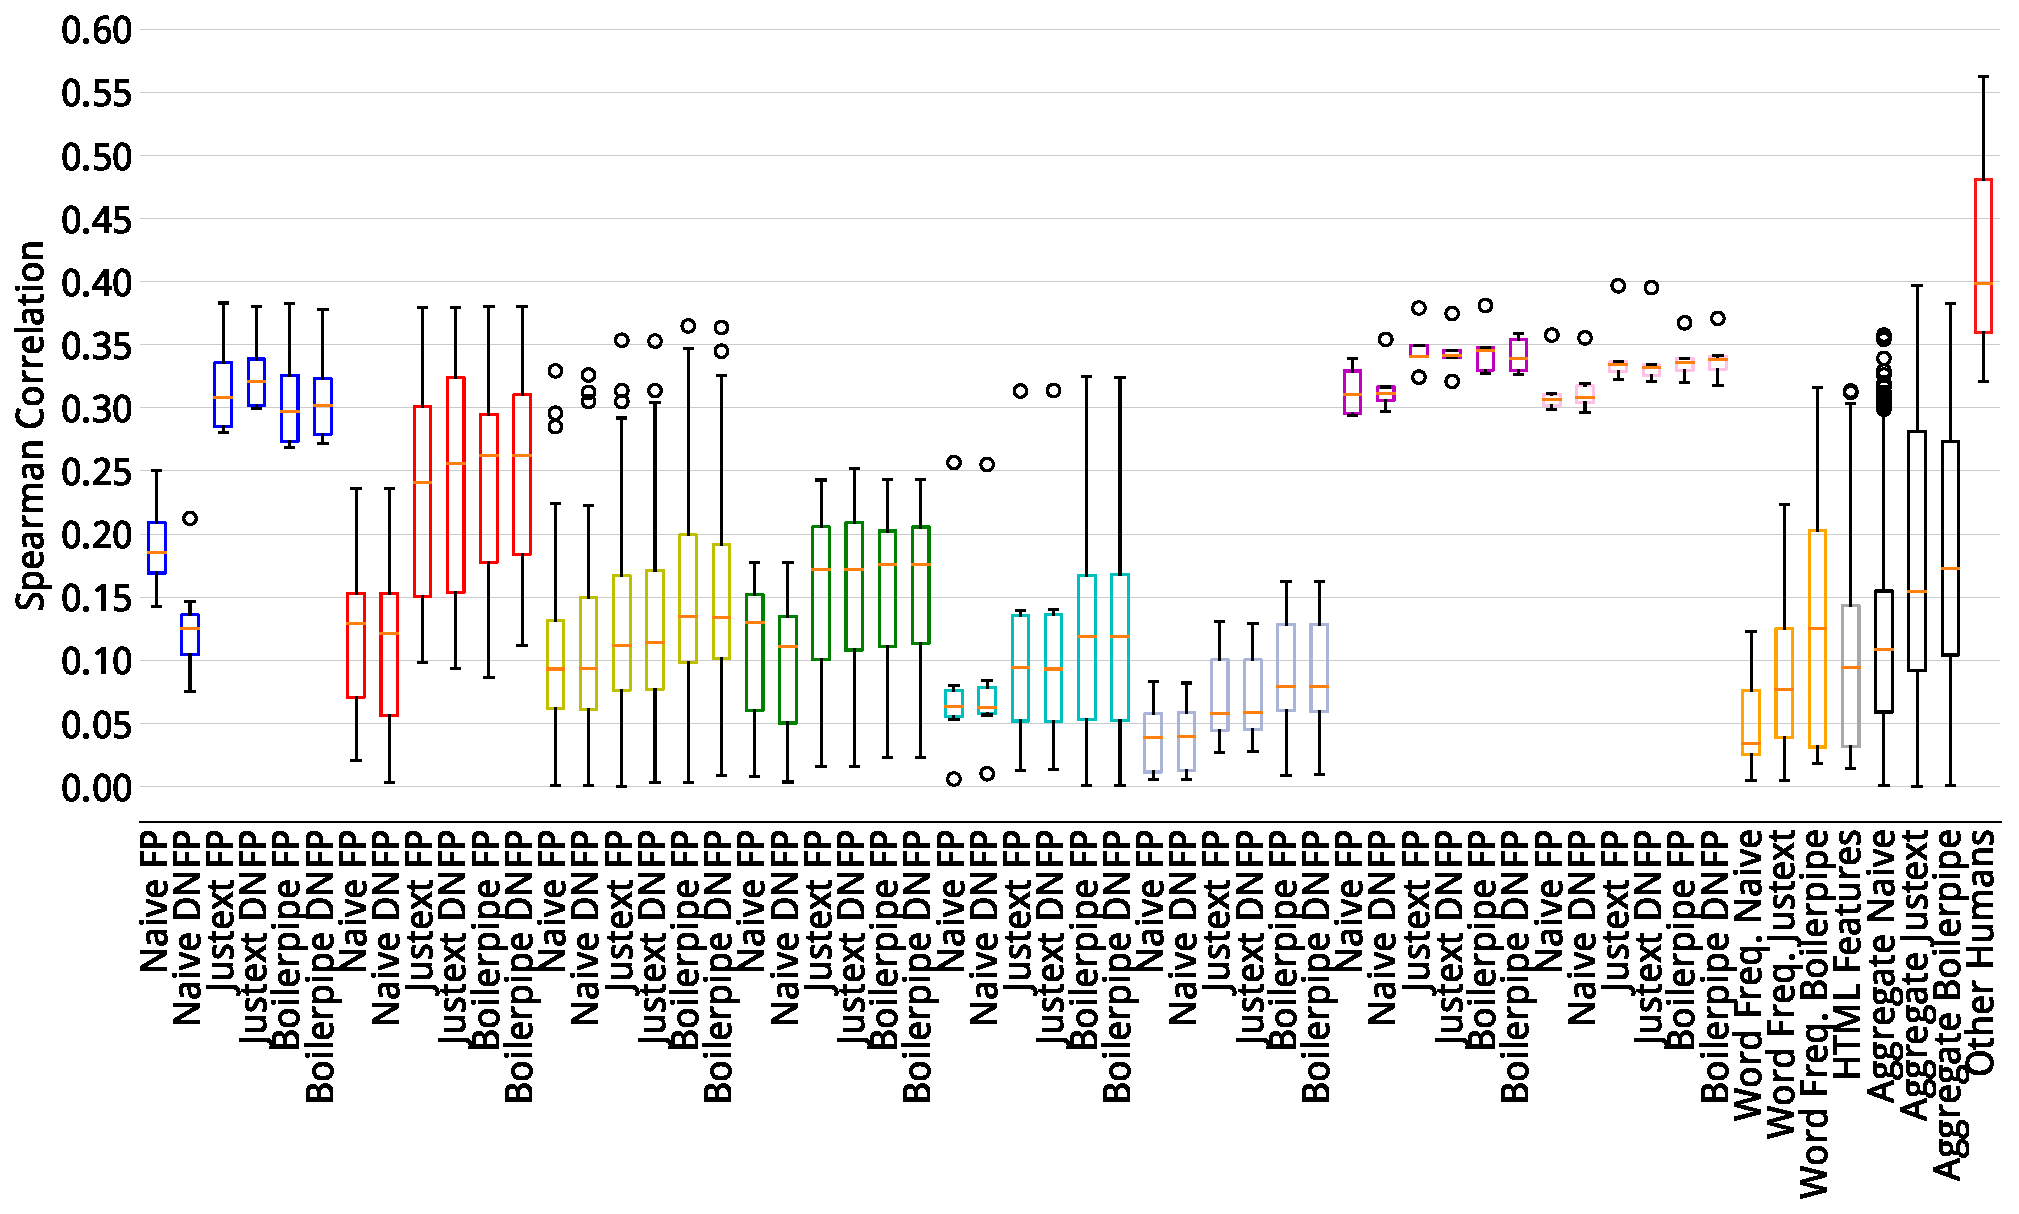
\includegraphics[width=0.6\textwidth]{graphics/box_spearman16_raw_values}
   %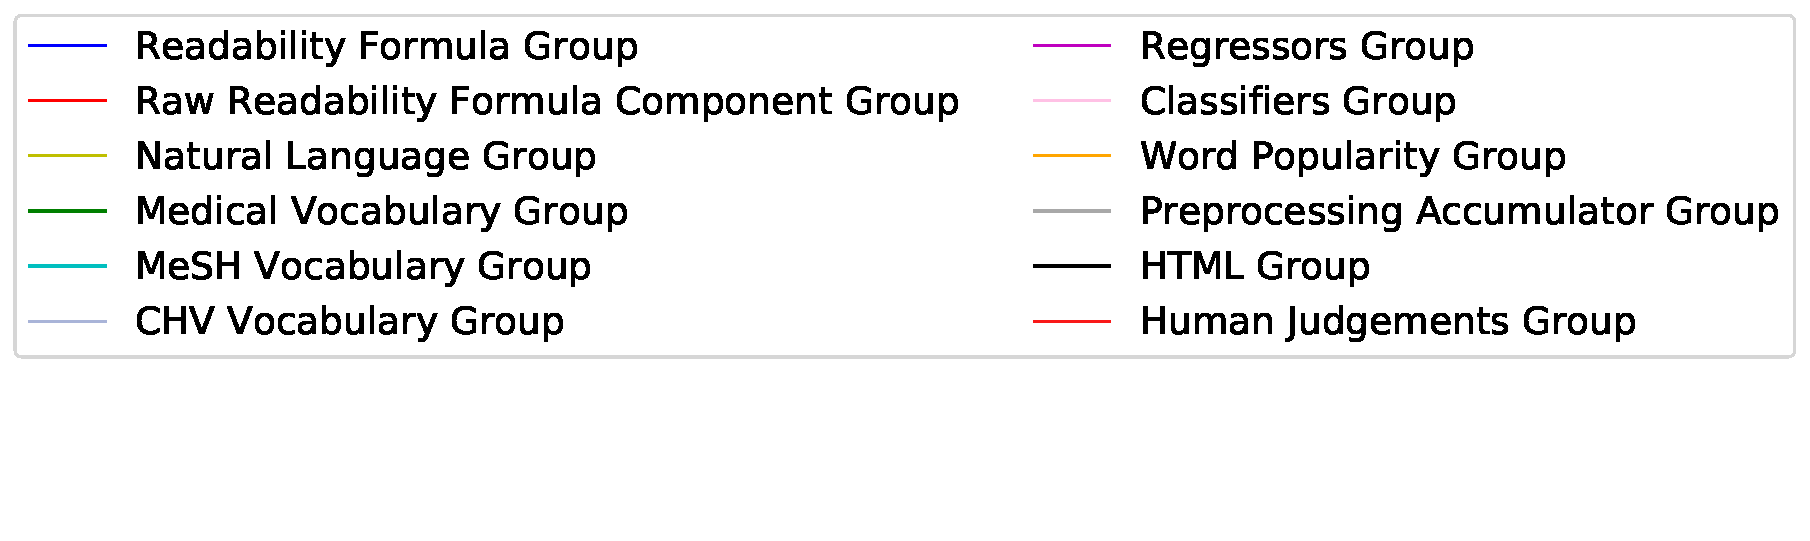
\includegraphics[width=0.7\textwidth]{graphics/legendCorr}
   \vspace{-0.4cm}
   \caption{Correlations between understandability estimators and human assessments for CLEF 2015 (top) and 2016 (bottom).}
   \label{fig:boxplot_corr_docs}
   \vspace{-10pt}
\end{figure*}

%
%\begin{figure*}[th!]
%   \centering
%   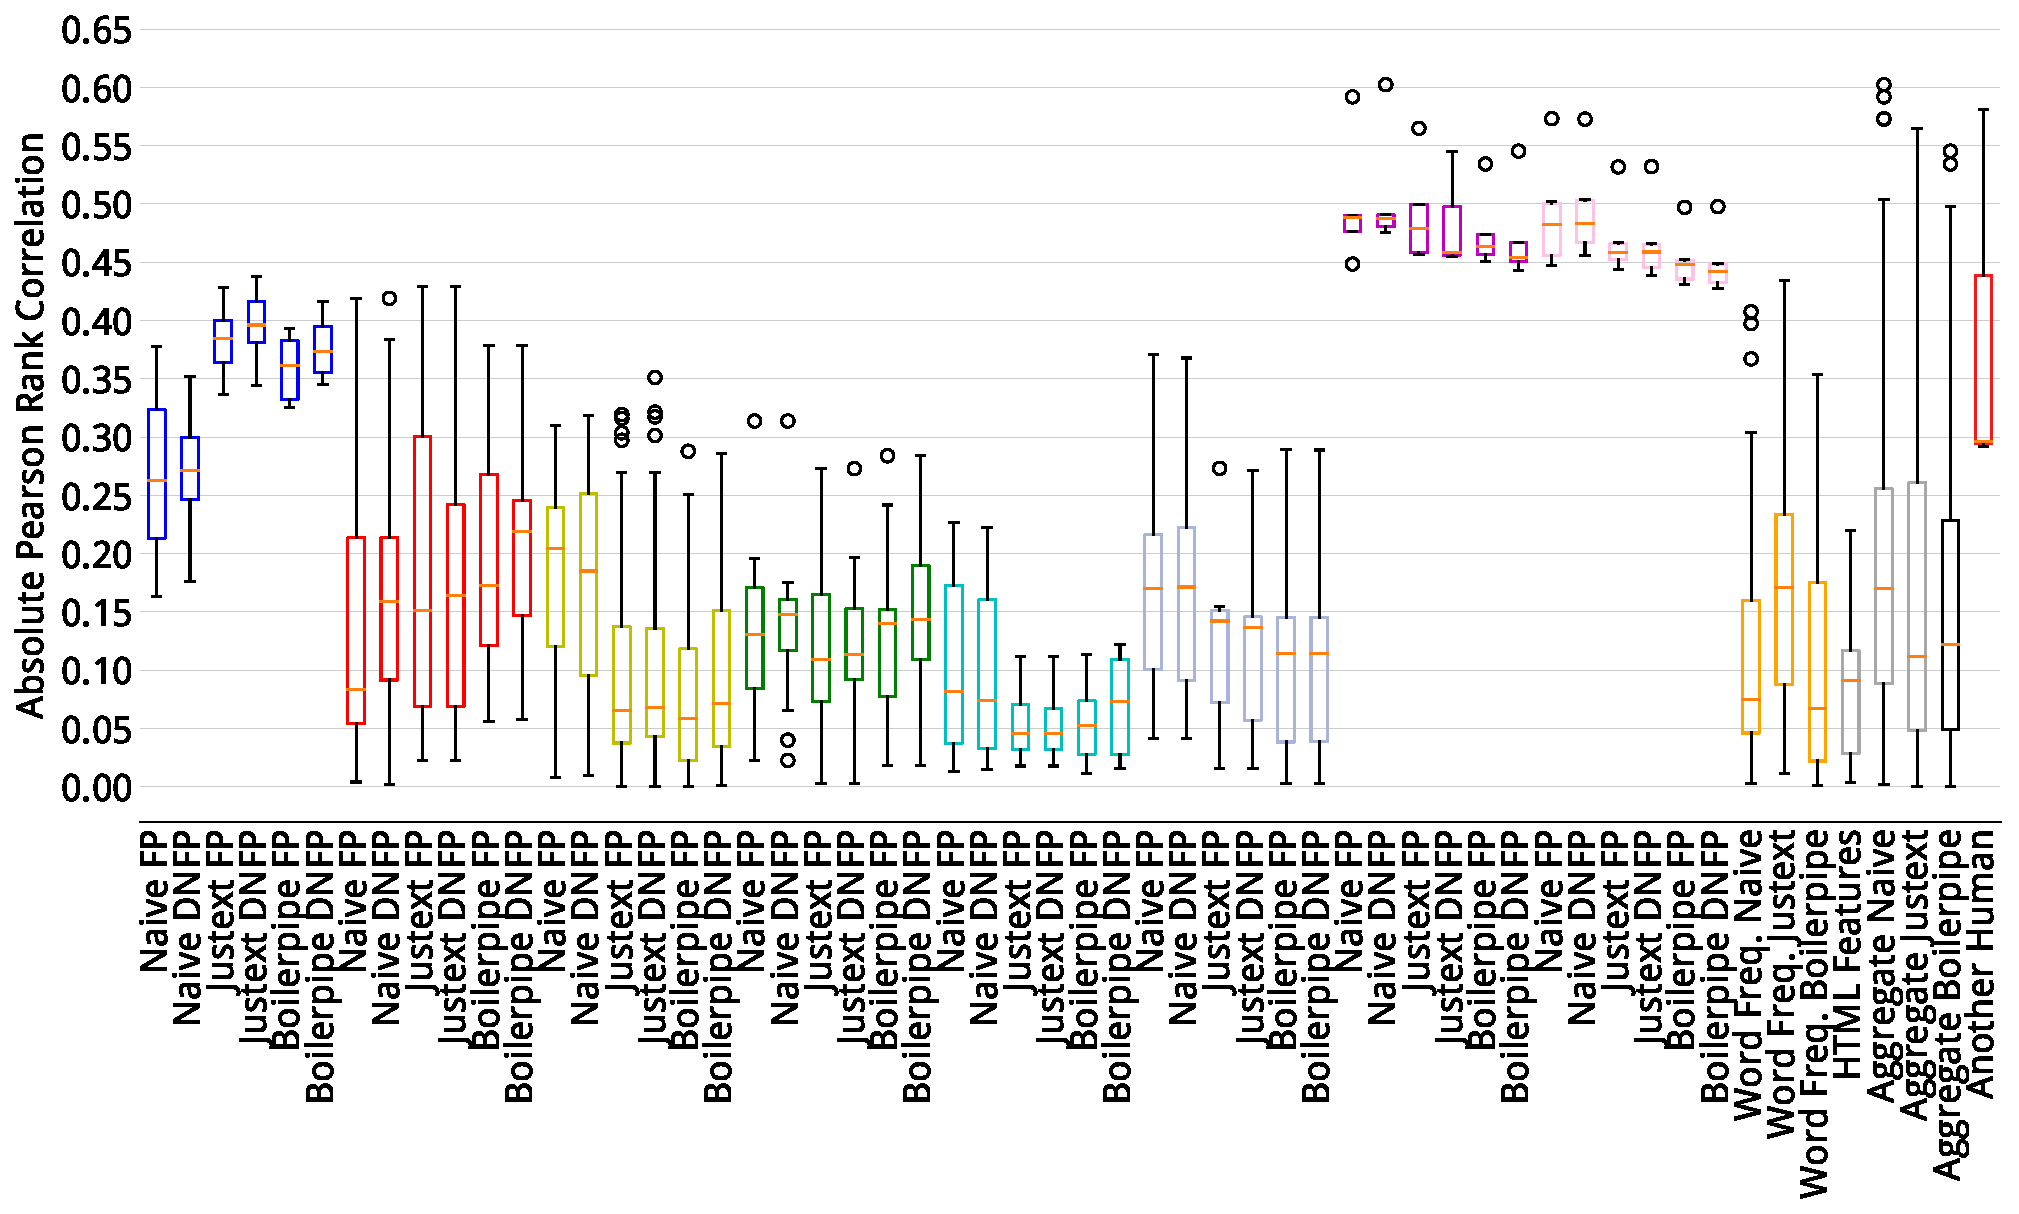
\includegraphics[width=0.90\textwidth]{graphics/box_pearson15_raw_values}
%   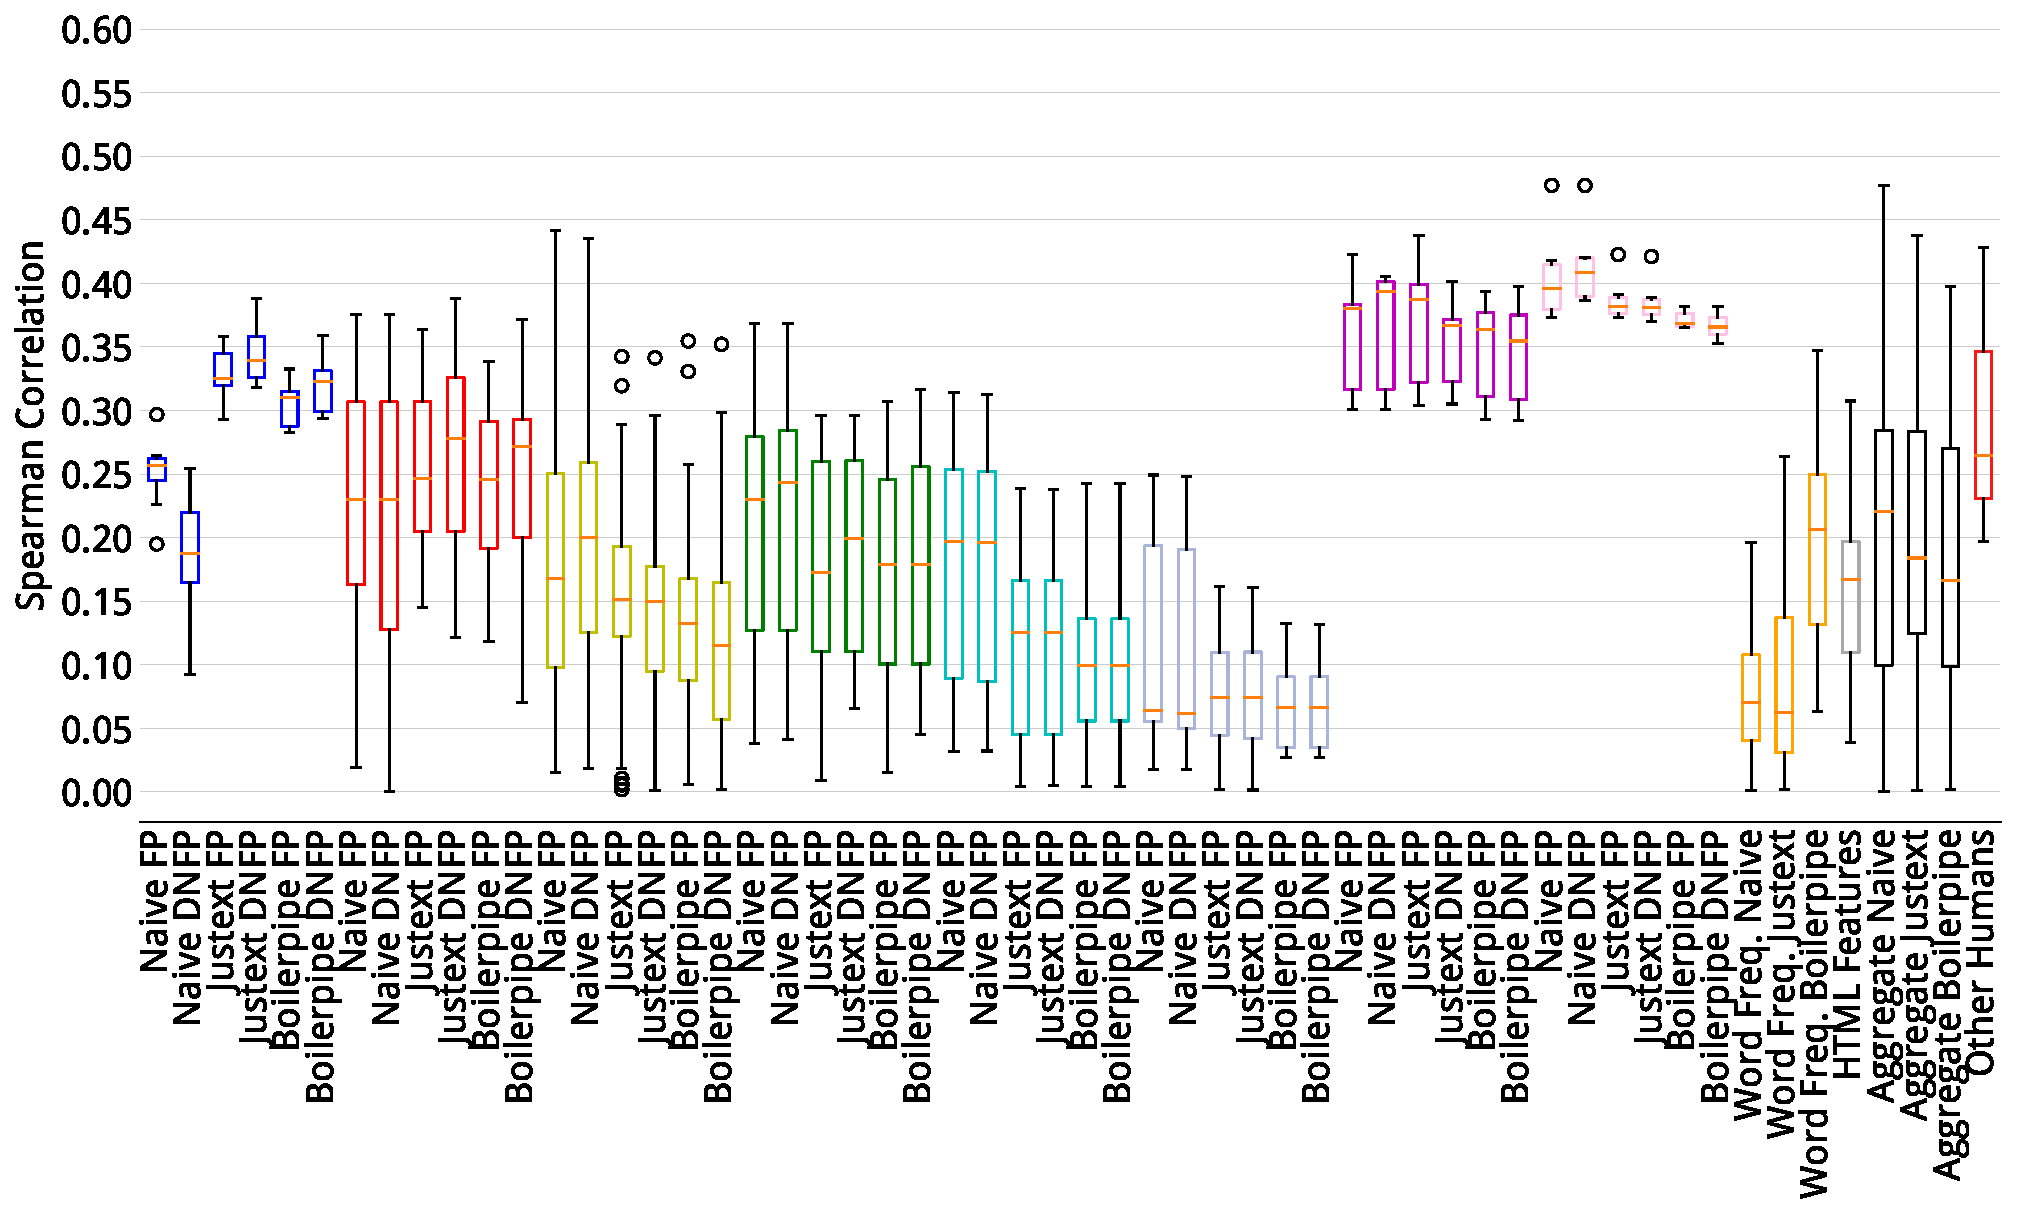
\includegraphics[width=0.90\textwidth]{graphics/box_spearman15_raw_values}
%   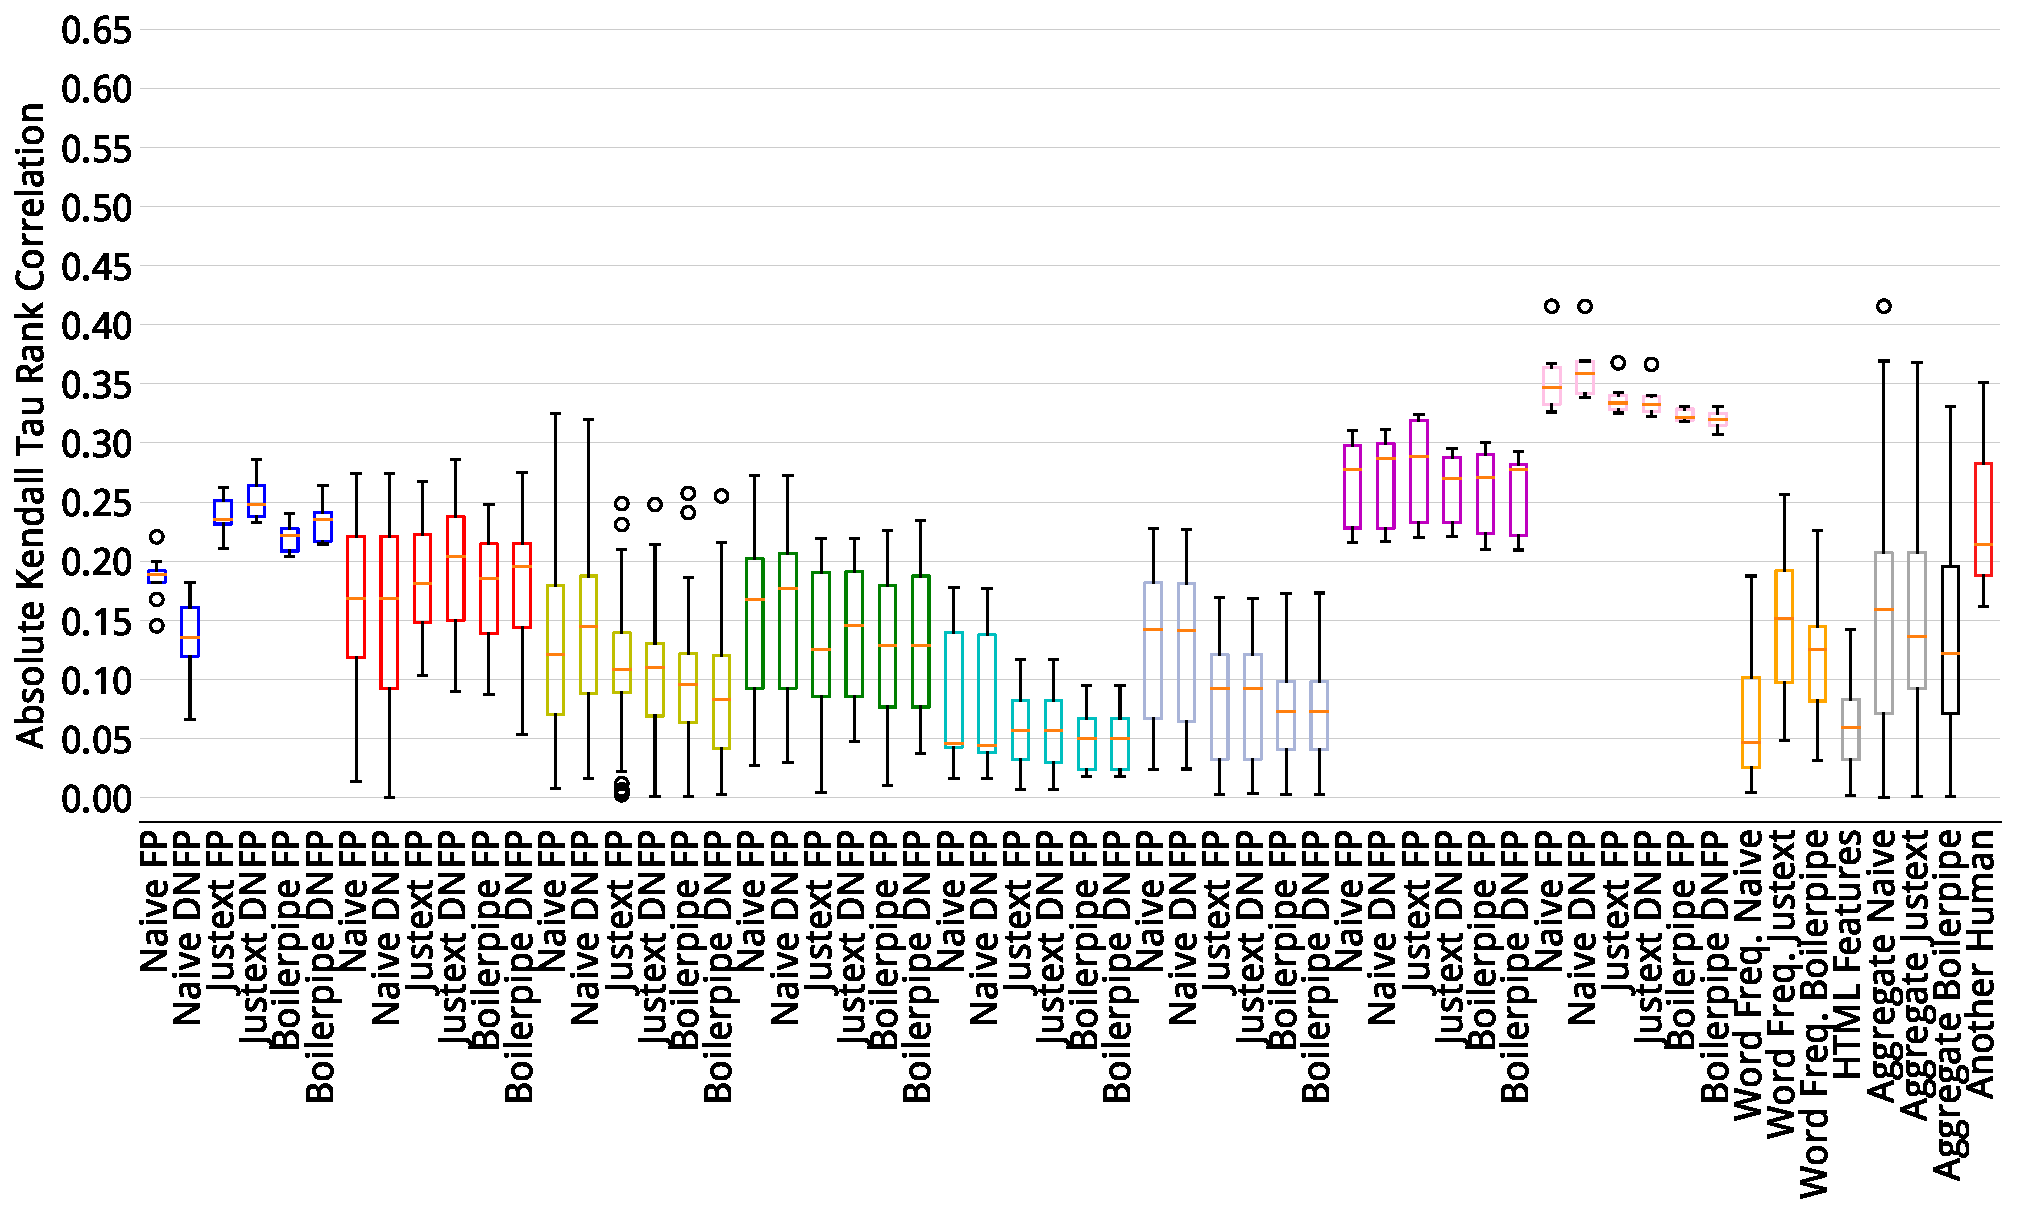
\includegraphics[width=0.90\textwidth]{graphics/box_kendalltau15_raw_values}
%   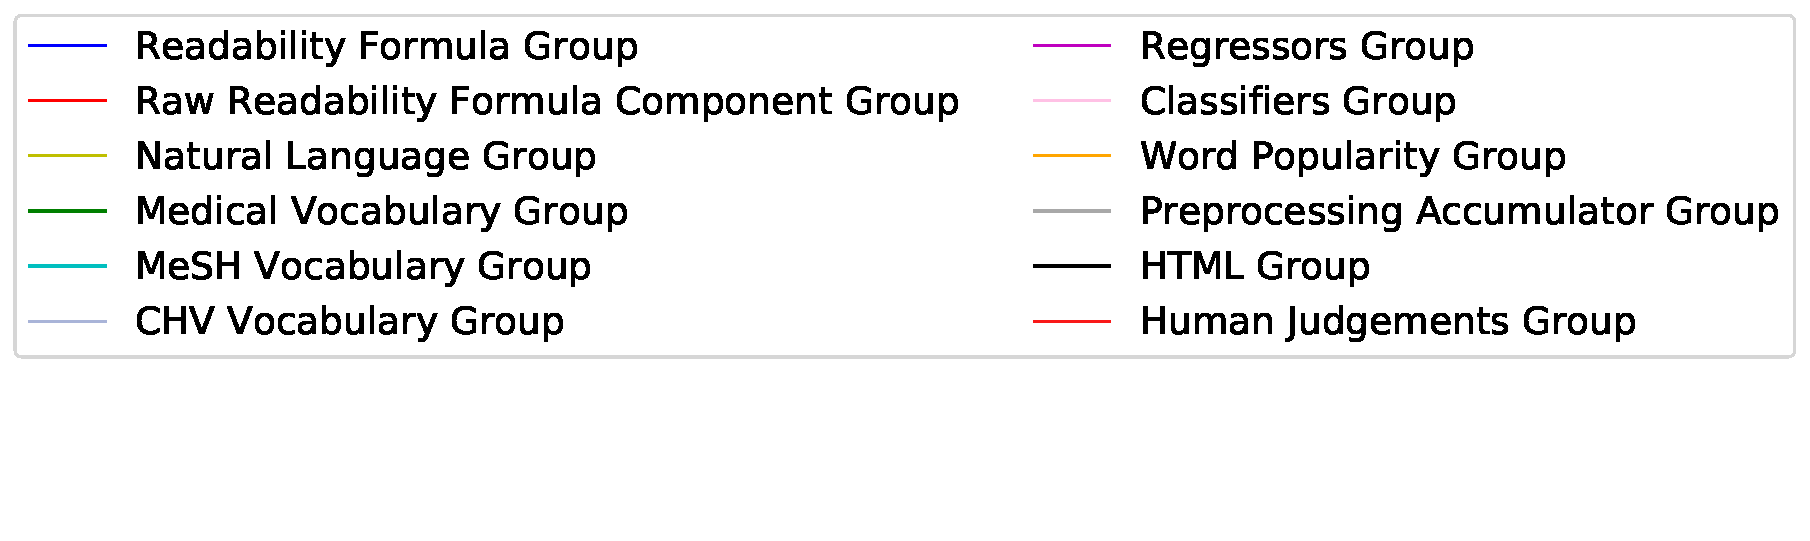
\includegraphics[width=0.65\textwidth]{graphics/legendCorr}
%   \caption{Box plots divided by feature groups. Correlations are calculated using understandability labels from relevant documents assessed in CLEF eHealth 2015}
%   \label{fig:boxplot_corr_docs_2015}
%\end{figure*}

%\begin{figure*}[th!]
%   \centering
%   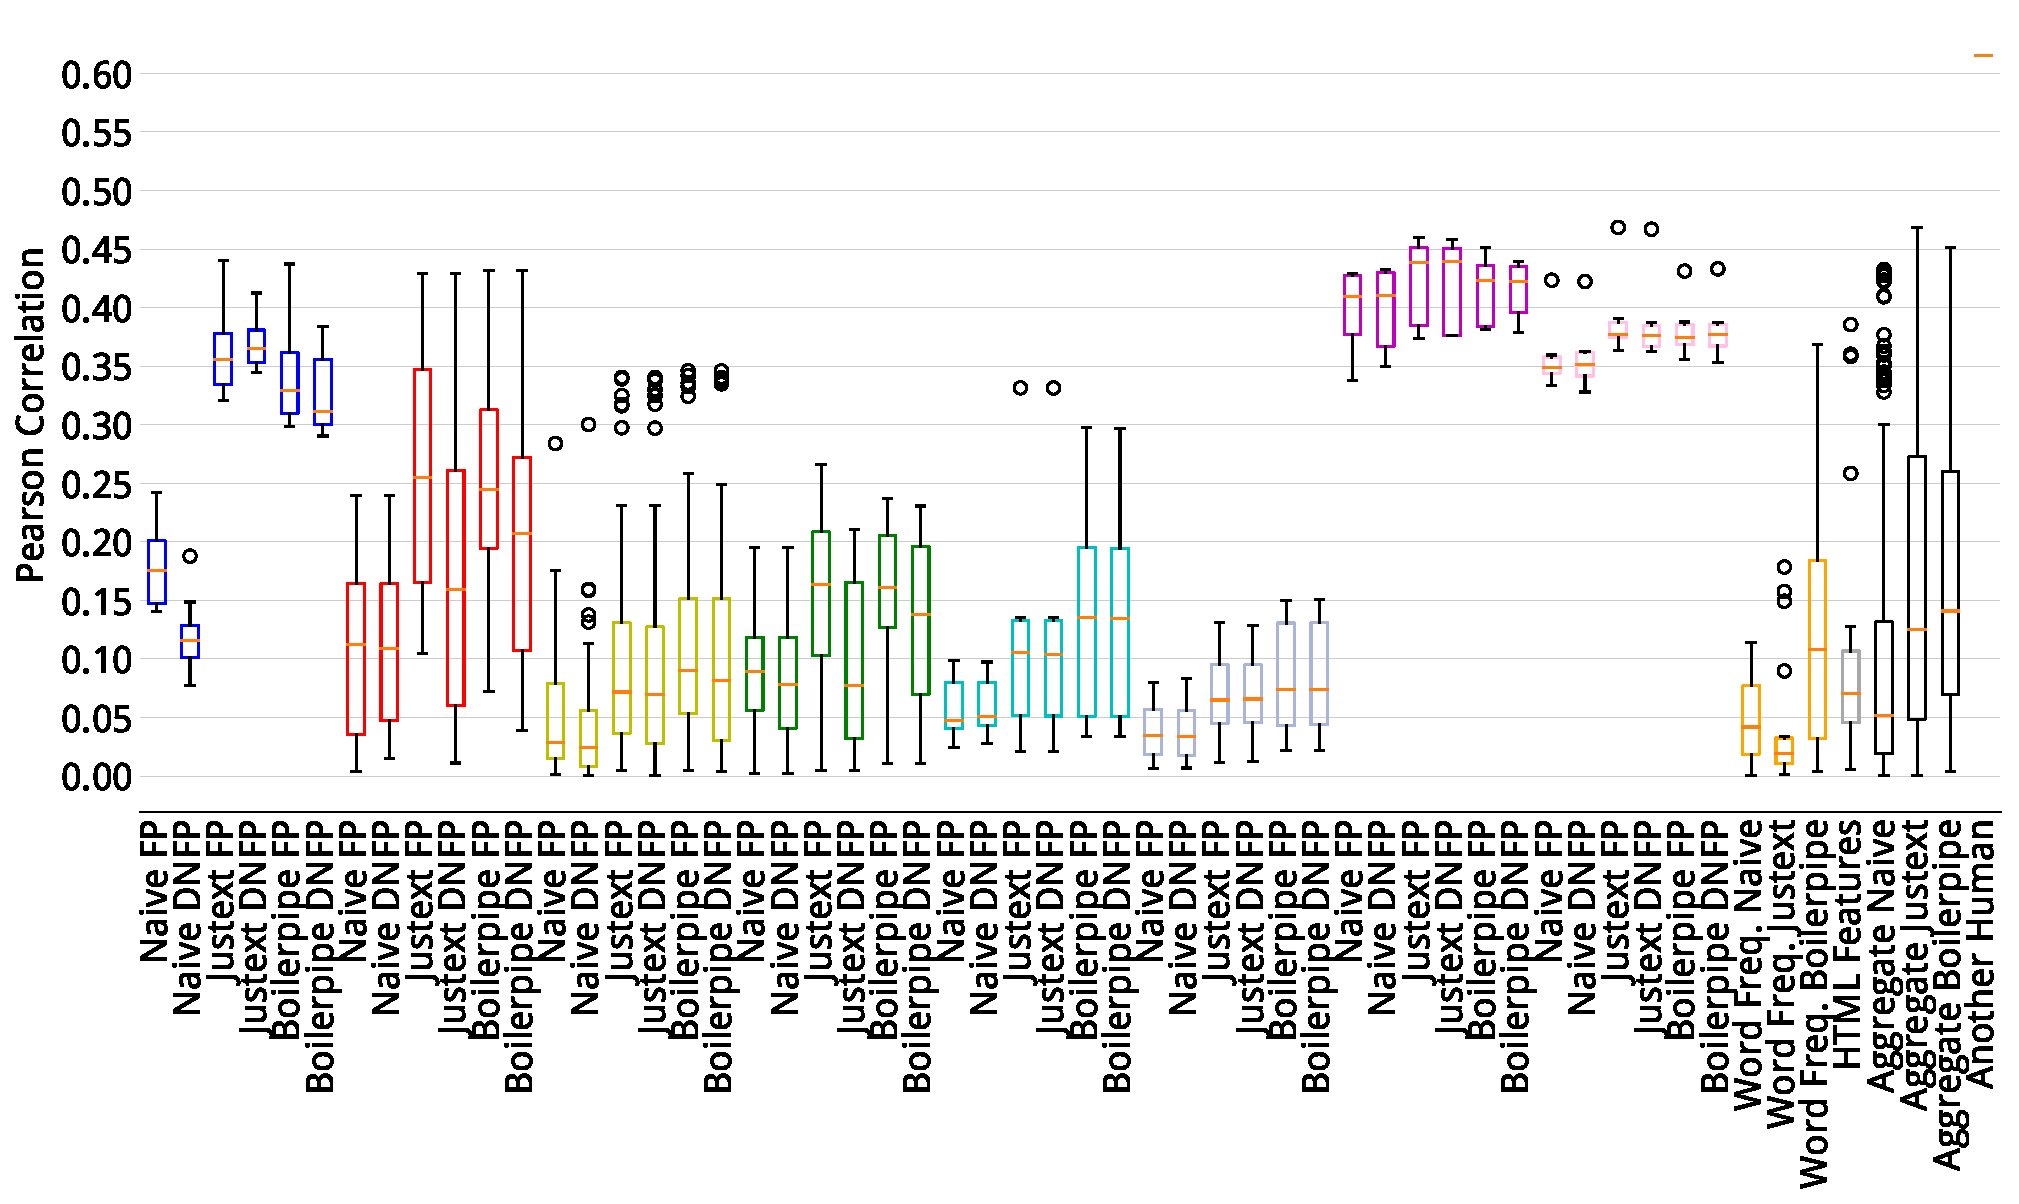
\includegraphics[width=0.90\textwidth]{graphics/box_pearson16_raw_values}
%   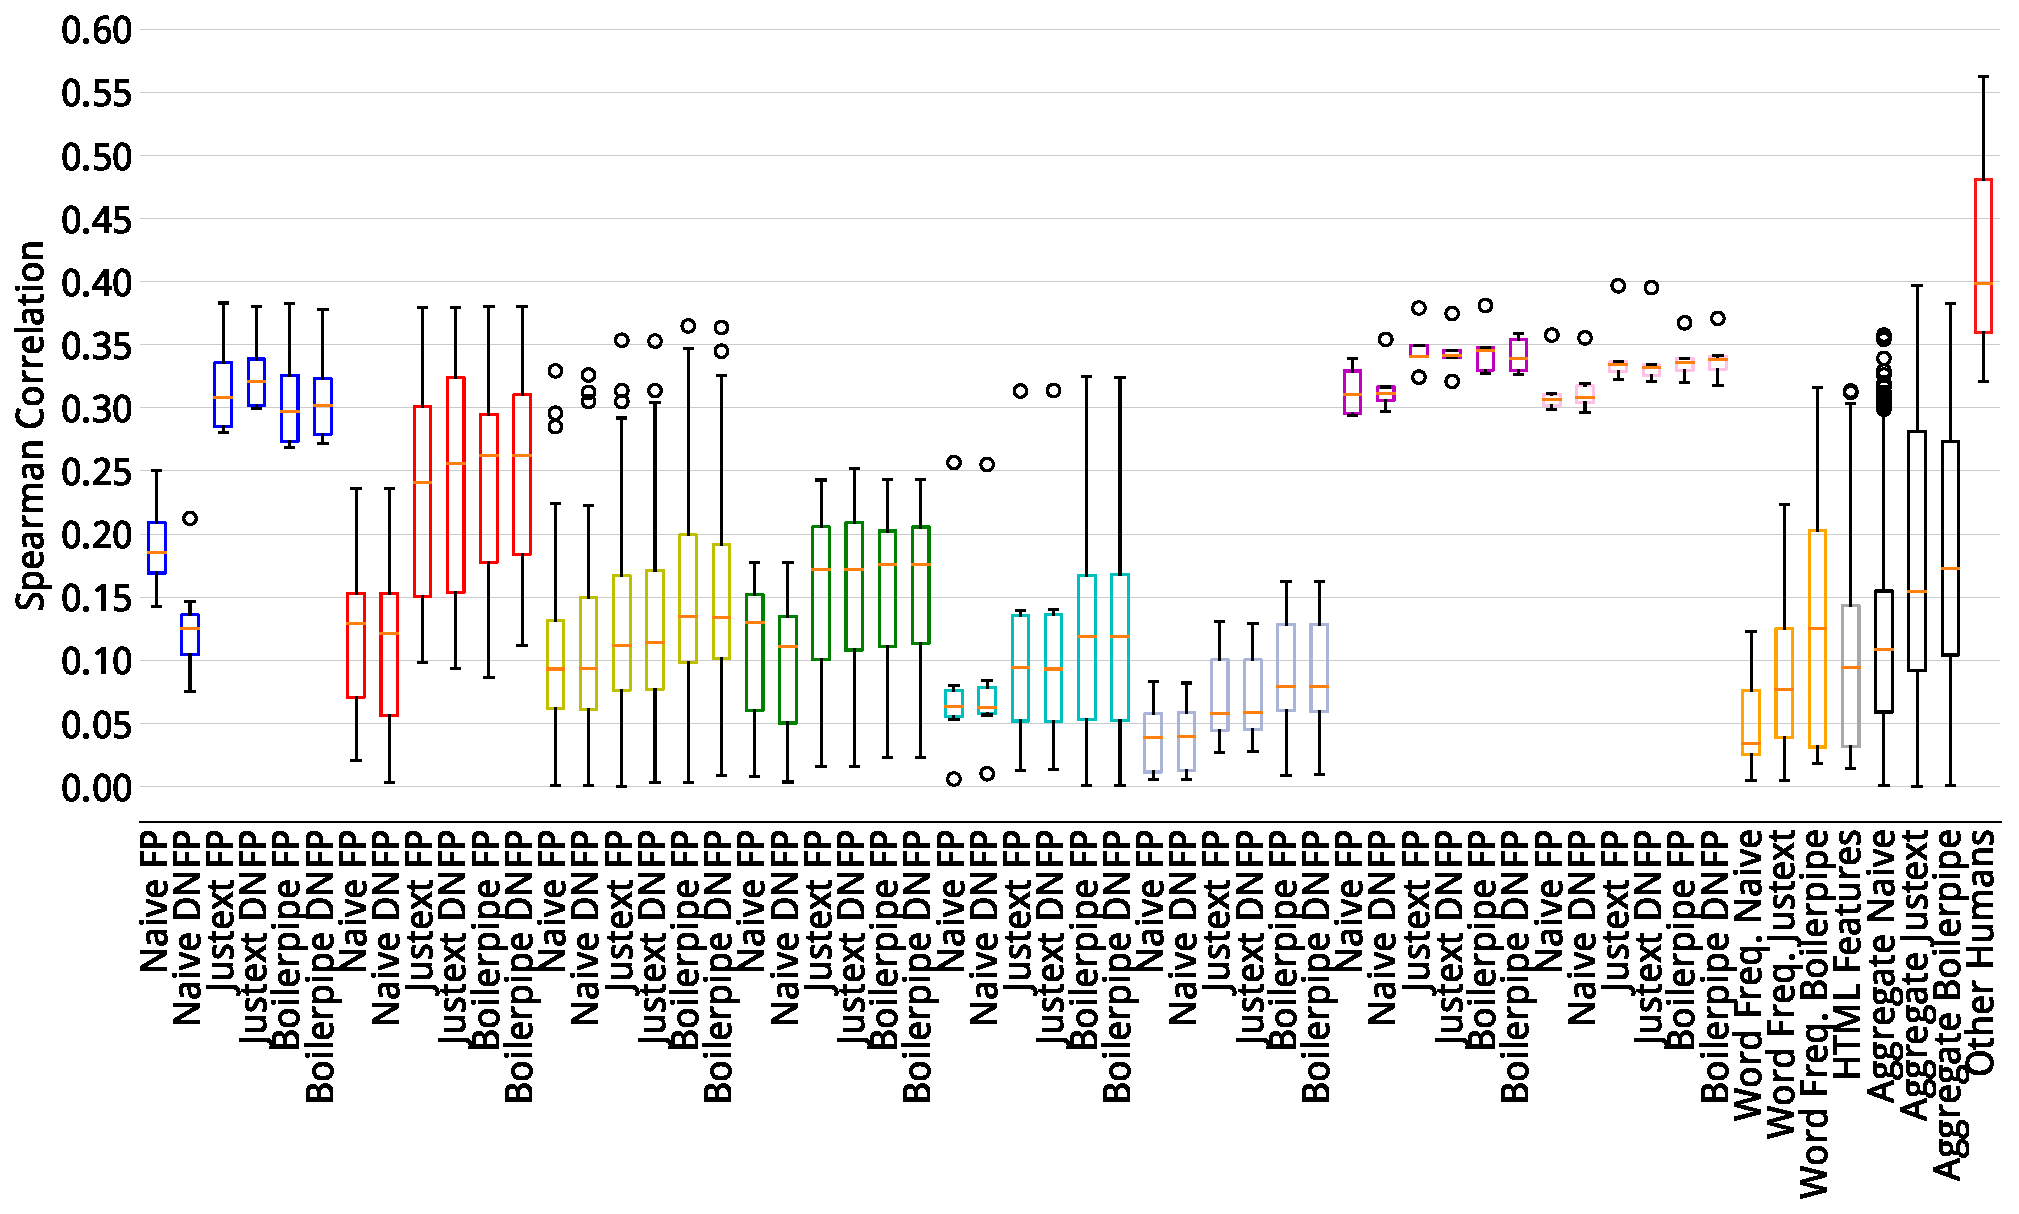
\includegraphics[width=0.90\textwidth]{graphics/box_spearman16_raw_values}
%   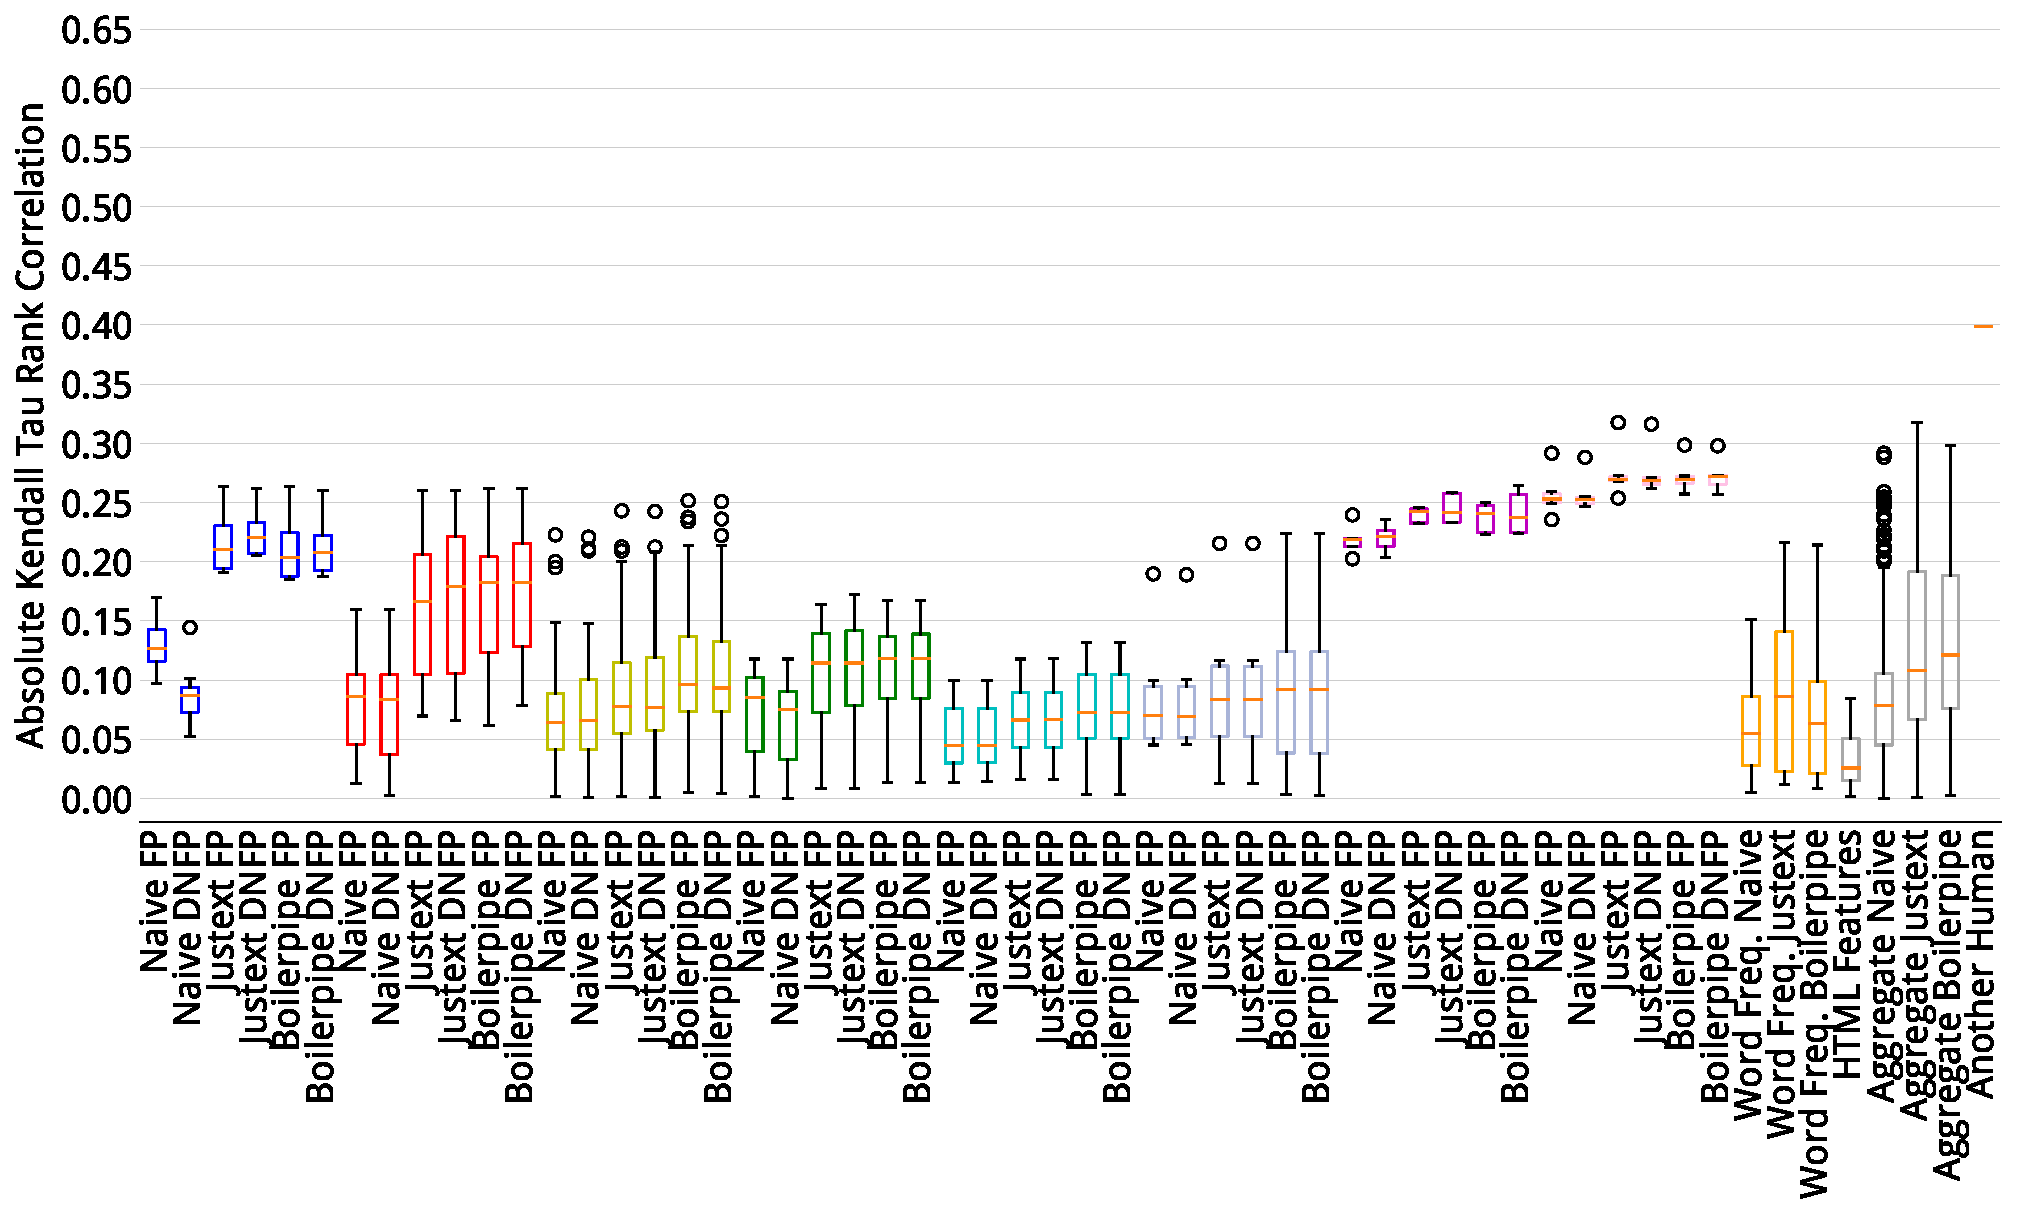
\includegraphics[width=0.90\textwidth]{graphics/box_kendalltau16_raw_values}
%    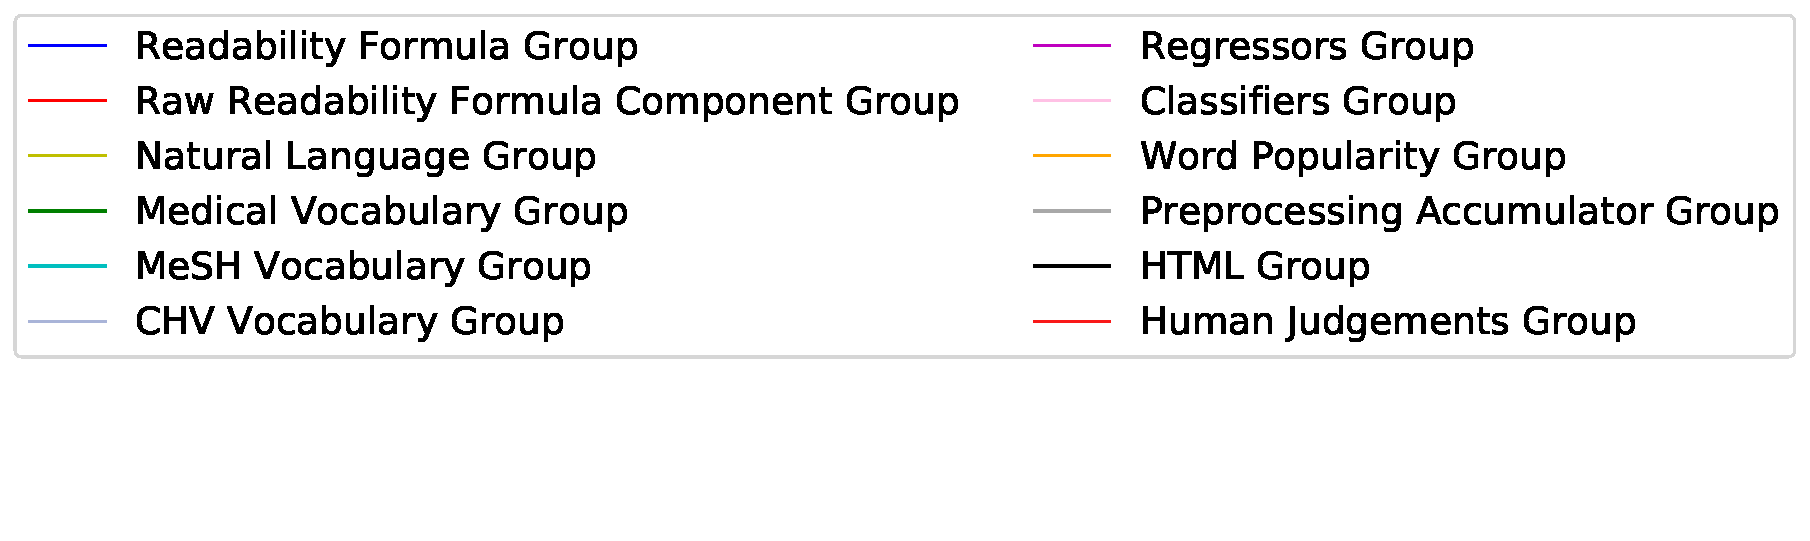
\includegraphics[width=0.65\textwidth]{graphics/legendCorr}
%    \caption{Box plots divided by feature groups. Correlations are calculated using understandability labels from relevant documents assessed in CLEF eHealth 2016}
%   \label{fig:boxplot_corr_docs_2016}
%\end{figure*}

%Figure~\ref{fig:boxplot_corr_docs_2015} shows the correlations for CLEF eHealth 2015 assessments.
%Top part of Figure~\ref{fig:boxplot_corr_docs} shows the Spearman correlation for CLEF eHealth 2015 assessments.

%The choice of preprocessing method had the highest impact on the traditional readability formula group, with the Naive preprocessing clearly underperforming the other preprocessing methods. The choice of the Naive method was also the worst for the word frequency group, but, interestingly, it was a good choice, or at least a competitive one, for all other groups.
%The highest correlations were archived by the regressors and classifiers, independently of the preprocessing method used.

%For this group, all correlation measures point out that the Naive processing yielded the weakest correlation, and Justext was marginally better than Boilerpipe. Comparing the medians, the strategy of DoNotForcePeriod performed better than ForcePeriod. The readability formula group was also the one with higher correlation, with an average correlation equal or higher than the human one.

%Similarly to Figure~\ref{fig:boxplot_corr_docs_2015}, Figure~\ref{fig:boxplot_corr_docs_2016} reports the findings for CLEF eHealth 2016. 
%Similarly the bottom part of Figure~\ref{fig:boxplot_corr_docs} reports the findings for CLEF eHealth 2016. 
%This time, though, the Naive preprocessing method was clearly underperforming for most of the groups analysed, including regressors and classifiers.

%In order to further understand our experiments, we compared the median of each pair of preprocessing strategy showed in Figures~\ref{fig:boxplot_corr_docs_2015} and~\ref{fig:boxplot_corr_docs_2016} and present the results in Table~\ref{tab:comparison_preprocessing}. 

%%% Removed because of space:
%%%We further analysed the results by performing pairwise comparisons between the median correlations across preprocessing pipelines and heuristics, and reporting the number of times the median correlation of a setting was better than another. These are reported in Table~\ref{tab:comparison_preprocessing}: in brackets we reported the number of comparisons that were statistically significant. 

%%% We first examined the comparison between sentence ending heuristics (ForcePeriod (FP) and DoNotForcePeriod (DNFP)). Results showed that the two methods achieved comparable results. Then we examined the comparison between preprocessing pipelines. For these, results for CLEF 2015 were in contrast with those for CLEF 2016. While Naive was marginally better than Boilerpipe and Justext in 2015, it was the worst in the majority of comparisons for 2016. In turn, while Justext was significantly better than Boilerpipe in 2015, they showed balanced results in 2016.
% \todo{I think something could be said about ustext and Boilerpipe. Done.}
 
%\begin{table}
\centering    
\caption{Exhaustive Comparison summary using the data from Figures 1.2 and 1.3. Numbers inside parentheses represent the number of tests that yielded p < 0.05 in a two-tailed t-test}
\label{tab:comparison_preprocessing}

\resizebox{1.\textwidth}{!}{
\begin{tabular}{lllllllll}
\toprule
\multirow{2}{*}{\textbf{Comparison}} & \multicolumn{4}{c}{\textbf{CLEF 2015}} & \multicolumn{4}{c}{\textbf{CLEF 2016}}\tabularnewline
\cmidrule(l{2pt}r{2pt}){2-5} \cmidrule(l{2pt}r{2pt}){6-9} 
& \textbf{Pearson} & \textbf{Spearman} & \textbf{Kendall Tau} & \textbf{Total} & \textbf{Pearson} & \textbf{Spearman} & \textbf{Kendall Tau} & \textbf{Total}\tabularnewline
\midrule
FP > DNFP & 8 (0) & 11 (4) & 11 (3) & 30 (7) & 16 (10) & 10 (3) & 11 (4) & 37 (17)\tabularnewline
FP < DNFP & 16 (5) & 12 (5) & 12 (6) & 40 (16) & 8 (0) & 12 (2) & 11 (2) & 31 (4)\tabularnewline
FP == DNFP & 0 & 1 & 1 & 2 & 0 & 2 & 2 & 4\tabularnewline
\midrule
Naive > Justext & 11 (7) & 9 (6) & 9 (5) & 29 (18) & 1 (0) & 0 (0) & 0 (0) & 1 (0)\tabularnewline
Naive < Justext & 6 (4) & 8 (4) & 8 (4) & 22 (12) & 16 (12) & 17 (13) & 17 (13) & 50 (38)\tabularnewline
Naive == Justext & 0 & 0 & 0 & 0 & 0 & 0 & 0 & 0\tabularnewline
Naive > Boilerpipe & 12 (7) & 10 (6) & 10 (5) & 32 (18) & 0 (0) & 0 (0) & 0 (0) & 0 (0)\tabularnewline
Naive < Boilerpipe & 5 (4) & 7 (3) & 7 (3) & 19 (10) & 16 (12) & 17 (13) & 17 (13) & 51 (39)\tabularnewline
Naive == Boilerpipe & 0 & 0 & 0 & 0 & 0 & 0 & 0 & 0\tabularnewline
Justext > Boilerpipe & 10 (7) & 16 (9) & 14 (8) & 40 (24) & 9 (4) & 9 (4) & 4 (2) & 17 (8)\tabularnewline
Justext < Boilerpipe & 7 (2) & 1 (0) & 3 (1) & 11 (3) & 8 (2) & 8 (2) & 13 (2) & 34 (6)\tabularnewline
Boilerpipe == Justext & 0 & 0 & 0 & 0 & 0 & 0 & 0 & 0\tabularnewline
\bottomrule 
\end{tabular}
} % close resizebox
\end{table}

%


